\documentclass{beamer}
\usepackage[T1]{fontenc}
\usepackage{caption}
\captionsetup{font=scriptsize}
\usetheme{boxes}
\pagestyle{empty}

\AtBeginSection[]{
  \begin{frame}
  \vfill
  \centering
  \begin{beamercolorbox}[sep=8pt,center,shadow=true,rounded=true]{title}
    \usebeamerfont{title}\insertsectionhead\par%
  \end{beamercolorbox}
  \vfill
  \end{frame}
}

\addtobeamertemplate{navigation symbols}{}{%
    \usebeamerfont{footline}%
    \usebeamercolor[fg]{footline}%
    \hspace{1em}%
    \insertframenumber/\inserttotalframenumber
}

\title{Introduction to using the Unix shell}
\author{Damiano Ravalico}
\institute{University of Trieste}
\date{A.Y. 2022/2023}

\begin{document}

\begin{frame}
\maketitle
\end{frame}

\section{Fundamental concepts}
\begin{frame}
\frametitle{Users and Groups}
\begin{definition}
Every \alert{user} of the system has a unique login name (\emph{username}) and a corresponding numeric user ID (\emph{UID}).
\end{definition}
\end{frame}

\begin{frame}
\frametitle{Users and Groups}
For each user, these are defined by a line in the system password file, \textbf{/etc/passwd}, which includes the following additional information:
\begin{itemize}
\item \emph{Group ID:} group ID of the first of the groups of which the user is a member
\item \emph{Home directory:} the initial directory into which the user is placed after logging in
\item \emph{Login shell:} the name of the program to be executed to interpret user commands
\end{itemize}
\end{frame}

\begin{frame}
\frametitle{Users and Groups}
\begin{definition}
A \alert{group} is a set of users, divided into it for for administrative purposes (i.e. for controlling access to files and other system resources). 
\end{definition}
\end{frame}

\begin{frame}
\frametitle{Users and Groups}
Each group is identified by a single line in the system group file, \textbf{/etc/group}, which contains:
\begin{itemize}
\item \emph{Group name:} the (unique) name of the group
\item \emph{Group ID (GID):} the numeric ID associated with this group
\item \emph{User list:} a comma-separated list of login names of users who are members of this group
\end{itemize}
\end{frame}

\begin{frame}
\frametitle{Users and Groups}
\begin{definition}
There is a one special user, known as \alert{superuser}, that has special privileges within the system; its account has \emph{ID 0}. The superuser bypasses all permission checks in the system.
\end{definition}
\end{frame}

\section{Unix filesystem}
\begin{frame}
\frametitle{Single Directory Hierarchy}
\begin{itemize}
\item The kernel maintains a single hierarchical directory structure to organize all files in the system
\item At the base there is the root directory, named \textbf{/} (slash)
\item All files and directories are children or descendants of the root directory
\end{itemize}
\end{frame}

\begin{frame}
\frametitle{Example}
\begin{figure}[h]
\centering
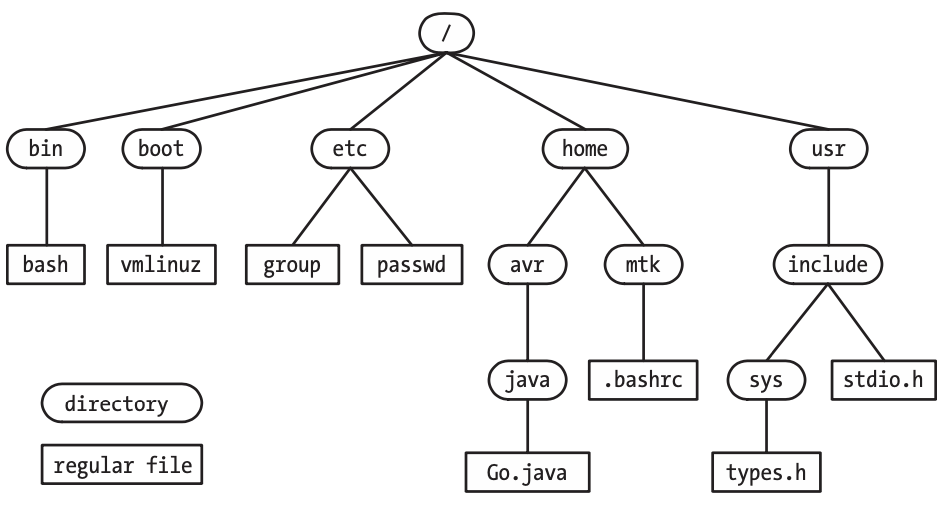
\includegraphics[width=10cm]{images/unix_filesystem.png}
\caption{Example of unix filesystem organization}
\end{figure}
\end{frame}

\begin{frame}
\frametitle{Files and types}
\begin{itemize}
\item Within the file system, each file is marked with a \alert{type}, indicating what kind of file it is (e.g. \textbf{.txt}).
\item Ordinary data files are usually called \alert{regular}
\item Note that the term \emph{file} is commonly used to denote a file of any type, not just a regular file
\end{itemize}
\end{frame}

\begin{frame}
\frametitle{Directories and Links}
\begin{definition}
A \alert{directory} is a special file whose contents take the form of a table composed of couples in the form \{filenames, references\} to the corresponding files; this association is called \alert{link}.
\\
Filenames can be up to 255 characters long and may contain any characters except slashes (\textbf{/}) and null characters (\textbackslash0).
\end{definition}
\end{frame}

\begin{frame}
\frametitle{Directories and Links}
\begin{itemize}
\item Directories may contain links both to files and to other directories
\item Every directory contains at least two entries: \emph{.} (dot), which is a link to itself, and \emph{..} (dot-dot), which is a link to its parent directory
\end{itemize}
\end{frame}

\begin{frame}
\frametitle{Pathnames}
\begin{definition}
A \alert{pathname} is a string consisting of an \emph{optional} initial slash (/) followed by a series of filenames separated by slashes. All but the last of these component filenames identifies a directory: it may identify any type of file, including a directory.
\end{definition}
\end{frame}

\begin{frame}
\frametitle{Pathnames}
\begin{itemize}
\item \alert{Absolute pathname} begins with a slash (/) and specifies the location of a file with respect to the root directory
\item \alert{Relative pathname} specifies the location of a file relative to the current directory 
\end{itemize}
\end{frame}

\section{Shell and Terminal Emulator}
\begin{frame}
\frametitle{What is shell?}
\begin{definition}
\alert{Shell} is a special-purpose program that reads text commands entered by the user, interprets them and passes them to the underlying operating system, in particular the kernel.
\end{definition}

\begin{definition}
\alert{Terminal emulator} is a program that opens a GUI (Graphical User Interface) to allow interaction with the shell.
\end{definition}

In most Linux distributions the default textual shell is called \alert{Bash}.
\end{frame}

\begin{frame}
\frametitle{In practice}
A command is a sequence of characters ending with the newline symbol (\emph{enter} key). These commands are predefined; they can be run alone, combined in a pipeline, or combined within a script.
\newline

Bash allows you to execute an \alert{pipeline} of commands, where the output of the previous command is the input of the next command.
\end{frame}

\section{File Permission and Access Modes}
\begin{frame}
\frametitle{File Permissions}
For the purpose of accessing a file, the system divides users into three categories:
\begin{itemize}
\item \emph{Owner} of the file
\item \emph{Group:} users who are members of the group matching the file’s group ID
\item \emph{Others:} the rest of the world
\end{itemize}
\end{frame}

\begin{frame}
\frametitle{Access Modes}
Three permission bits may be set for each of these categories (a total of nine permission bits):
\begin{itemize}
\item \emph{Read:} user can read the contents of the file
\item \emph{Write:} user can modify the contents of the file
\item \emph{Execute:} user can execute the file (typically a script or program)
\end{itemize}
\end{frame}

\begin{frame}
\frametitle{Access Modes}
If the file is a directory there are some differences:
\begin{itemize}
\item Read permission allows the contents of (i.e., the filenames in) the directory to be listed
\item Write permission allows the contents of the directory to be changed (i.e., filenames can be added, removed, and changed)
\item Execute permission allows access to files within the directory
\end{itemize}
\end{frame}

\begin{frame}
\frametitle{Symbolic notation}
Using the \textbf{ls -l} command in the terminal, it is possible to view the access modes of the files. This notation is called \alert{symbolic notation}.
\end{frame}

\begin{frame}
\frametitle{Symbolic notation}
The first character indicates the file type and is not related to permissions. The remaining nine characters are in three sets, each representing a class of permissions as three characters. 
\begin{itemize}
\item The first set represents the user category
\item The second set represents the group category
\item  The third set represents the others category
\end{itemize}
\end{frame}

\begin{frame}
\frametitle{Symbolic notation}
Each of the three characters represent the permissions:
\begin{itemize}
\item \textbf{r} if reading is permitted, \textbf{-} if it is not
\item \textbf{w} if writing is permitted, \textbf{-} if it is not
\item \textbf{x} if execution is permitted, \textbf{-} if it is not
\end{itemize}
\end{frame}

\begin{frame}
\frametitle{Symbolic notation - examples}
\begin{example}
\begin{itemize}
\item \textbf{-rwxr-xr-x}: a regular file whose user category has full permissions and whose group and others categories have only the read and execute permissions
\item \textbf{dr-x------}: a directory whose user category has read and execute permissions and whose group and others categories have no permissions
\end{itemize}
\end{example}
\end{frame}

\begin{frame}
\frametitle{Octal notation}
\begin{table}[!h]
\begin{center}
\begin{tabular}{ ccc } 
\hline
Binary value & Octal value & Permissions \\
(\textbf{rwx}) & & \\
\hline
000 & 0 & none \\
001 & 1 & execution only \\
010 & 2 & writing only \\
011 & 3 & writing and execution \\
100 & 4 & read only \\
101 & 5 & reading and execution \\
110 & 6 & reading and writing \\
111 & 7 & read, write and execute \\
\hline
\end{tabular}
\caption{Permission representations}
\end{center}
\end{table}
\end{frame}

\section{Main commands}
\begin{frame}
\frametitle{Command format}
\textbf{command\_name [option(s)] [parameter(s)]}
\begin{itemize}
\item \textbf{command\_name:} is the name of the command to perform
\item \textbf{option}: modifies a command’s operation. To invoke it, use hyphens (–) or double hyphens (—)
\item \textbf{parameter:} specifies any necessary information for the command
\end{itemize}

Note that:
\begin{itemize}
\item A command may contain an option or a parameter
\item Commands are case-sensitive
\end{itemize}
\end{frame}

\begin{frame}
\frametitle{List}
\textbf{ls}: lists the contents of the current directory
\newline
\begin{example}
\begin{itemize}
\item \textbf{ls *.pdf} lists all files ending with the suffix .pdf located in the current directory
\item \textbf{ls -a} shows hidden files in addition to the visible ones
\item \textbf{ls -lh} shows the file sizes in easily readable formats
\end{itemize}
\end{example}
\end{frame}

\begin{frame}
\frametitle{Change directory}
\textbf{cd}: changes the current folder to the specified one
\newline
\begin{example}
\begin{itemize}
\item \textbf{cd} change the current directory to the home of the current user
\item \textbf{cd /temp} change the current directory to \textbf{temp}
\item \textbf{cd ..} moves one directory up
\end{itemize}
\end{example}
\end{frame}

\begin{frame}
\frametitle{Concatenate}
\textbf{cat}: lists, combines, and writes file content to the standard output
\begin{example}
\begin{itemize}
\item \textbf{cat filename.txt} displays content
\item \textbf{tac filename.txt} displays content in reverse order
\end{itemize}
\end{example}
\end{frame}

\begin{frame}
\frametitle{Copy}
\textbf{cp}: copies files or directories and their content
\begin{example}
\begin{itemize}
\item To copy one file from the current directory to another, enter \textbf{cp} followed by the file name and the destination director
\item To copy files to a directory, enter the file names followed by the destination directory
\item \textbf{cp -R dir\_to\_copy /destination/path/} copies the directory and the entire subtree connected at that point in the specified path
\end{itemize}
\end{example}
\end{frame}

\begin{frame}
\frametitle{Create directory}
\textbf{mkdir}: creates one or multiple directories at once
\begin{example}
\textbf{mkdir test} creates a directory named \textbf{test} in the current directory
\end{example}
\end{frame}

\begin{frame}
\frametitle{Remove}
\textbf{rm}: deletes file and directory
\begin{example}
\begin{itemize}
\item \textbf{rm filename1 filename2} deletes all three files
\item \textbf{rm -r} delete an entire folder (even if not empty)
\end{itemize}
\end{example}
\end{frame}

\begin{frame}
\frametitle{Create and modify files}
\textbf{touch}: creates an empty file with the specified name

\textbf{nano}: allows users to edit and manage files via text editor

\textbf{vi}: another text editor, standard, unlike \textbf{nano} which is only present in some linux distros
\end{frame}

\begin{frame}
\frametitle{Change mode}
\textbf{chmod}: modifies a file or directory’s read, write, and execute permissions
\begin{example}
\textbf{chmod 777 test.md} changes the file permissions to the \textbf{-rwxrwxrwx} permission type, whose numeric value is 777 
\end{example}
\end{frame}

\begin{frame}
\frametitle{User manual}
\textbf{man command\_name} provides a user manual of any commands or utilities you can run in Terminal, including the name, description, and options. To exit from it, press \emph{q}.
\newline

\begin{figure}[h]
\centering
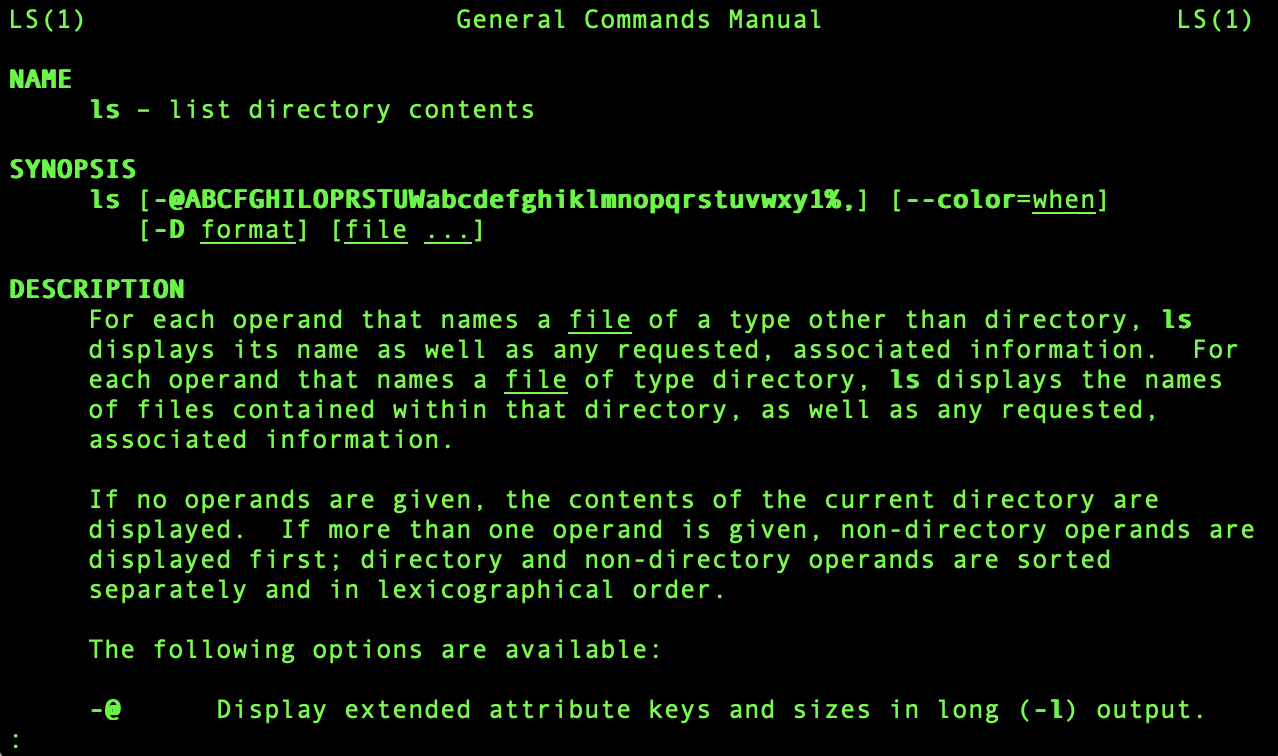
\includegraphics[width=7cm]{images/man_ls.png}
\caption{First page of the \textbf{ls} command manual}
\end{figure}
\end{frame}

\section{Pipes}

\begin{frame}
\frametitle{File descriptors}
\begin{definition}
A \alert{file descriptor} is a non-negative integer representing any type of file opened by a process and on which the process can perform input/output operations. Each process has its own set of file descriptors.
\end{definition}
\end{frame}

\begin{frame}
\frametitle{File descriptors}
\begin{table}[!h]
\begin{center}
\begin{tabular}{ cc } 
\hline
File descriptor & Purpose \\
\hline
0 & standard input \\
1 & standard output \\
2 & standard error \\
\hline
\end{tabular}
\caption{Standard file descriptors}
\end{center}
\end{table}
\end{frame}

\begin{frame}
\frametitle{Pipe}
\begin{definition}
An \alert{pipe} is a tool that allows processes to communicate with each other. In particular, it is a method for linking the stdout of one program to the stdin of the next.
\end{definition}
\end{frame}

\begin{frame}
\frametitle{Pipe}
\begin{itemize}
\item A pipe is a unidirectional communication channel
\item A pipe is a byte stream: there is no concept of messages or message boundaries when using a pipe
\item Pipes have a limited capacity
\item To concatenate commands use the \textbf{|}, to redirected the stdout of a command to a file use the \textbf{>}
\end{itemize}
\end{frame}

\begin{frame}
\frametitle{Pipe - example}
\textbf{ls | wc -l}
\begin{itemize}
\item In order to execute the above command, the shell creates two processes, executing \textbf{ls} and \textbf{wc}
\item \textbf{ls} lists the file in the current directory
\item \textbf{|} symbol indicates that the output of the first command is the input of the second
\item \textbf{wc -l} uses that list to print the number of lines (\textbf{-l} option) i.e. the length of the list in this case 
\end{itemize}
\end{frame}

\end{document}